\documentclass[10pt,a4paper]{article}
\usepackage[utf8]{inputenc}
\usepackage{verbatim}
\usepackage{amsmath}
\usepackage{amsthm}
\usepackage{amssymb}
\usepackage{amsfonts}
\usepackage{amssymb}
\usepackage{mathrsfs}
\usepackage{mathtools}
\usepackage{graphicx}
\usepackage{geometry}
\usepackage{framed}
\usepackage{enumitem}
\usepackage{tabto}
\usepackage{xcolor}
\usepackage{tikz}
\usepackage{tkz-euclide}
\usepackage{enumitem}   

\usetikzlibrary{arrows}
\usetikzlibrary{calc}

\usetkzobj{angles}





\newtheorem{theorem}{\color{red}{Teorema}}[section]
\newtheorem{lemma}[theorem]{\color{purple!70}{Lema}}
\newtheorem{proposition}[theorem]{\color{purple!70}{Proposição}}
\newtheorem{conjecture}[theorem]{\color{purple!70}{Conjectura}}
\newtheorem{corollary}[theorem]{\color{purple!70}{Corolário}}
\newtheorem{definition}[theorem]{\color{blue!90}{Definição}}

\newtheorem{remark}[theorem]{\color[rgb]{0,.5,0}{Observação}}
\newtheorem{attention}[theorem]{\color[rgb]{.75,0,0}{Atenção}}

\renewcommand*{\proofname}{Demonstração}

\newcommand{\bref}[1]{\textsuperscript{\tiny\textnormal{\textbf{\setlength{\fboxsep}{1pt}\colorbox{gray!50}{\color{white}{#1}}}}}}

%\endinput



\geometry{
	a4paper,
	total={210mm,297mm},
	left=20mm,
	right=20mm,
	top=15mm,
	bottom=15mm,
}

\setlist[description]{leftmargin=\parindent,labelindent=\parindent,topsep=0pt,itemsep=-1ex,partopsep=1ex,parsep=1ex}
\setlist[itemize]{leftmargin=\parindent,labelindent=\parindent,topsep=0pt,itemsep=-1ex,partopsep=1ex,parsep=1ex}
\setlist[enumerate]{leftmargin=\parindent,labelindent=\parindent,topsep=0pt,itemsep=-.4em,partopsep=1ex,parsep=1ex}

%\setlength\parindent{0pt}

\author{Gino Chen Hsiang-Jan}
\title{Resumo Álgebra Linear}
\date{26 de Outubro de 2015}

\begin{document}
\maketitle
\tableofcontents

\newpage

%******************************************************************************
% Projeção ortogonal
%******************************************************************************
\section{Projeção ortogonal}
\begin{definition}\bref{[Anton,AlgLinApl-pt,2010]}
Dizemos que dois vetores não nulos $u$ e $v$ em $\mathbb{R}^n$ são ortogonais (ou perpendiculares) se $u.v = 0$. Também convencionamos que o vetor nulo em $\mathbb{R}^n$ é ortogonal a cada vetor em $\mathbb{R}^n$. Um conjunto não vazio de vetores em $\mathbb{R}^n$ é denominado ortogonal se dois quaisquer de seus vetores forem ortogonais. Um conjunto ortogonal de vetores unitários é dito ortonormal.
\end{definition}

\begin{theorem}\bref{[Anton,AlgLinApl-pt,2010]}\\

(a) Se $a$ e $b$ constantes não ambas nulas, então uma equação da forma:\\
\[
	a x + b y + c = 0
\]
representa uma reta em $\mathbb{R}^2$ de normal $n = (a, b)$.\\

(b) Se $a$, $b$ e $c$ constantes não ambas nulas, então uma equação da forma:
\[
	a x + b y + c z + d = 0
\]
representa um plano em $\mathbb{R}^3$ de normal $n = (a, b, c)$.
\end{theorem}

\begin{theorem}\bref{[Anton,AlgLinApl-pt,2010]} \textbf{Teorema das projeções} Se $u, v \in \mathbb{R}^n$ e se $v \neq 0$, então $u$ pode ser escrito de maneira única na forma $u = w_1 + w_2$, em que $w_1$ é um múltiplo escalar de $v$ e $w_2$ é ortogonal a $v$.
\end{theorem}

\begin{definition}\bref{[Anton,AlgLinApl-pt,2010]} No teorema das projeções:\\
	$w_1$ é chamado de projeção ortogonal de $u$ ou componente vetorial de $u$ ao longo de $v$ e denotado como $proj_v u$ e pode ser calculado por: 
	\[
		w_1 = proj_v u = \frac{\langle u, v \rangle}{\langle v, v \rangle} v
	\]
	$w_2$ é chamado de componente vetorial de $u$ a $v$ e pode ser calculado por:
	\[
		w_2 = u - proj_v u = u - \frac{\langle u, v \rangle}{\langle v, v \rangle} v
	\]
\end{definition}

\begin{definition}\bref{[Anton,AlgLinApl-pt,2010]} Dizemos que um conjunto de dois ou mais vetores num espaço com produto interno é \textbf{ortogonal} se quaisquer dois vetores distintos do conjunto forem ortogonais.
\end{definition}

\begin{definition}\bref{[Anton,AlgLinApl-pt,2010]} Um conjunto ortogonal no qual cada vetor tem normal 1 é \textbf{ortonormal}.
\end{definition}

\begin{theorem}\bref{[Anton,AlgLinApl-pt,2010]} Se $\mathsf{S} = \{ v_1, v_2, v_3, \dots, v_n \}$ for um conjunto ortogonal de vetores não nulos num espaço com produto interno, então $\mathsf{S}$ é linearmente independente
\end{theorem}

\begin{theorem}\bref{[Anton,AlgLinApl-pt,2010]} Se $\mathsf{S} = \{ v_1, v_2, v_3, \dots, v_n \}$ for uma base ortogonal de espaço com produto interno $\mathsf{V}$ e $u \in \mathsf{V}$ então :
\[
	u = \frac{\langle u, v_1 \rangle}{\lVert v_1 \rVert ^ 2} v_1 + \frac{\langle u, v_2 \rangle}{\lVert v_2 \rVert ^ 2} v_2 + \frac{\langle u, v_3 \rangle}{\lVert v_3 \rVert ^ 2} v_3 + \dots + \frac{\langle u, v_n \rangle}{\lVert v_n \rVert ^ 2} v_n
\]
\end{theorem}

\begin{theorem}\bref{[Anton,AlgLinApl-pt,2010]} Se $\mathsf{S} = \{ v_1, v_2, v_3, \dots, v_n \}$ for uma base ortonormal de espaço com produto interno $\mathsf{V}$ e $u \in \mathsf{V}$ então :
\[
	u = \langle u, v_1 \rangle v_1 + \langle u, v_2 \rangle v_2 + \langle u, v_3 \rangle v_3 + \dots + \langle u, v_n \rangle v_n
\]
\end{theorem}

\begin{theorem}\bref{[Anton,AlgLinApl-pt,2010]} Seja $\mathsf{W}$ um subespaço de dimensão finita de um espaço vetorial com produto interno $\mathsf{V}$\\
(a) Se $\mathsf{S} = \{ v_1, v_2, v_3, \dots, v_n \}$ for uma base ortogonal de $\mathsf{W}$ e $u \in \mathsf{V}$ então :
\[
	u = \frac{\langle u, v_1 \rangle}{\lVert v_1 \rVert ^ 2} v_1 + \frac{\langle u, v_2 \rangle}{\lVert v_2 \rVert ^ 2} v_2 + \frac{\langle u, v_3 \rangle}{\lVert v_3 \rVert ^ 2} v_3 + \dots + \frac{\langle u, v_n \rangle}{\lVert v_n \rVert ^ 2} v_n
\]
(b) Se $\mathsf{S} = \{ v_1, v_2, v_3, \dots, v_n \}$ for uma base ortonormal de $\mathsf{W}$ e $u \in \mathsf{V}$ então :
\[
	u = \langle u, v_1 \rangle v_1 + \langle u, v_2 \rangle v_2 + \langle u, v_3 \rangle v_3 + \dots + \langle u, v_n \rangle v_n
\]
\end{theorem}

\begin{theorem}\bref{[Anton,AlgLinApl-pt,2010]} Cada espaço vetorial não nulo de dimensão finita possui alguma base ortonormal.
\end{theorem}

\begin{comment}
Projeção ortogonal de um ponto em uma reta.
Seja $\mathsf{V} = \mathbb{R}^2$ um espaço vetorial euclidiano, um plano. Dado uma reta $r$ e um ponto $P = (x_1, y_1)$ Desejamos encontrar um ponto $N = (x_0, y_0)$ que é projeção do ponto $P$ na reta $r$. Um ponto $N$ em $r$ que tem a menor distância entre a reta $r$ e o ponto $P$.\\

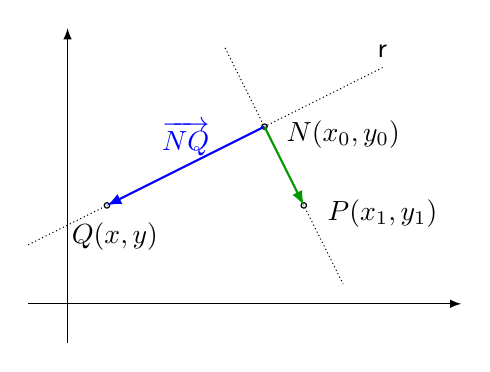
\begin{tikzpicture}[dot/.style={circle,inner sep=1pt,fill,label={#1},name=#1}, line/.style={>=latex}] 
	\coordinate (Q) at ( .5, 1.25) ;
	\coordinate (N) at (2.5, 2.25) ;
	\coordinate (P) at (3.0, 1.25);
	\coordinate (r1)  at (-.5, .75);
	\coordinate (r2) at (4, 3) ;
	\coordinate (s1)  at (2, 3.25);
	\coordinate (s2) at (3.5, 0.25) ;
	\node (QLabel) at ($(Q)+(.1,-.4)$) {$Q(x, y)$};
	\node (NLabel) at ($(N)+(1, -0.1)$) {$N(x_0, y_0)$};
	\node (PLabel) at ($(P)+(1, -0.1)$) {$P(x_1, y_1)$};
	\node (rLabel) at ($(r2)+(0, 0.2)$) {$\mathsf{r}$};
	\draw[->, line] (-.5, 0) -- (5, 0);
	\draw[->, line] (0, -.5) -- (0, 3.5);
	\draw[-, line, densely dotted] ($(r1)$) -- ($(r2)$);
	\draw[-, line, densely dotted] ($(s1)$) -- ($(s2)$);
	\tkzDrawPoints(Q, N, P)
	\draw[->, line, color=blue, thick] ($(N)$) -- node [above] {$\overrightarrow{NQ}$} ($(Q)$);
	\draw[->, line, color=green!60!black, thick] ($(N)$) -- ($(P)$);
	\draw (rLabel);
	\draw (QLabel);
	\draw (NLabel);
	\draw (PLabel);
\end{tikzpicture}

Para de terminar a direção de $r$, vamos escolher um ponto $Q = (x, y)$ em $r$, tal que $\overrightarrow{NQ} = (x - x_0, y - y_0)$ e $Q \neq N$. Então:
\[
	\overrightarrow{NQ} \perp \overrightarrow{NP} \Leftrightarrow \langle(x - x_0, y - y_0), (x_1 - x_0, y_1 - y_0)\rangle = 0
\]
\[
	x_0 ^ 2 - (x + x_1) x_0 + x x_1 + y_0 ^ 2 - (y + y_1) y_0 + y y_1 = 0 \Leftrightarrow
\]

Seja $\mathsf{V}$ um espaço vetorial de corpo $K$ munido de produto interno. $u, v \in \mathsf{V}$, $u \neq 0$ e $v \neq 0$. 
\end{comment}


%******************************************************************************
% Matrizes
%******************************************************************************
\section{Matrizes}

\begin{definition}\bref{[Noble,AlgLinApl-pt,1986]}
Chama-se de matriz transposta hermitiana, denotado por $A^H$, $A^H = \overline{A}^t$, que é a complexa cojugada da transposta ordinária.
\end{definition}

\begin{definition}\bref{[Noble,AlgLinApl-pt,1986]}
Chama-se de matriz hermitiana uma matriz tal que $A^H = A$.
\end{definition}

\begin{lemma}\bref{[Noble,AlgLinApl-pt,1986]}
Uma matriz hermitiana é a soma de uma matriz real simétrica e de uma matriz imaginária anti-simétrica.
\end{lemma}

\begin{lemma}\bref{[Noble,AlgLinApl-pt,1986]}
As propriedades de matrizes são válidas:
	\begin{itemize}
		\item $\overline{AB} = \overline{A}.\overline{B}$
		\item $(\overline{A})^t = (\overline{A^t})$
	\end{itemize}
\end{lemma}

\begin{definition}\bref{[Noble,AlgLinApl-pt,1986]}
	Uma matriz $P$ tal que $P^HP = PP^H = I$ é chamada matriz unitária. 
\end{definition}

\begin{definition}\bref{[Noble,AlgLinApl-pt,1986]}
	Uma matriz $P$ real tal que $P^TP = PP^T = I$ é chamada matriz ortogonal.
\end{definition}

\begin{theorem}\bref{[Noble,AlgLinApl-pt,1986]}
	\begin{enumerate}[label=(\roman*)]
		\item Tanto as colunas quanto as linhas de uma matriz unitária (ou ortogonal) formal um cojunto ortonormal.
		\item Se $P$ é unitária, então $|det P| = 1$.
		\item Se $P$ e $Q$ são unitárias, então o mesmo acontece com $PQ$.
		\item Se $P$ é unitária, então, para todos os $x$ e $y$, temos $(Px, Py), \lVert Px \rVert_2 = \lVert x \rVert_2$ e $\lVert P \rVert_2 = 1$.
		\item Se $\lambda$ for um autovalor da matriz unitária $P$, então $|\lambda| = 1$.
	\end{enumerate}
\end{theorem}

\begin{definition}\bref{[Noble,AlgLinApl-pt,1986]}
	Uma matriz quadrada $A$ que satisfaz $A^HA = AA^H$ é chamada matriz normal.
\end{definition}

\begin{lemma}\bref{[Noble,AlgLinApl-pt,1986]}
	Seja $A$ uma matriz quadrada.
	\begin{enumerate}[label=(\roman*)]
		\item Matrizes hermitianas são normais, ou seja $A^HA = AA^H = AA$
		\item Se $A$ é uma matriz real, $A^TA = AA^T = AA$, $A$ é simétrico.
	\end{enumerate}
\end{lemma}



%******************************************************************************
% Processo de Gram-Schmidt
%******************************************************************************
\section{Processo de Gram-Schmidt}
\bref{[Anton,AlgLinApl-pt,2010]} Para converter uma base $\{ u_1, u_2, u_3, \dots, u_n \}$ numa base ortogonal $\{ v_1, v_2, v_3, \dots, v_n \}$, efetue as seguintes contas:
\begin{flalign*}
& v_1 = u_1 &&\\\
& v_2 = u_2 - \frac{\langle u_2, v_1 \rangle}{\lVert v_1 \rVert ^ 2} v_1 &&\\
& v_3 = u_3 - \frac{\langle u_3, v_1 \rangle}{\lVert v_1 \rVert ^ 2} v_1 - \frac{\langle u_3, v_2 \rangle}{\lVert v_2 \rVert ^ 2} v_2&&\\
&\vdots&&\\
& v_n = u_n - \frac{\langle u_n, v_1 \rangle}{\lVert v_1 \rVert ^ 2} v_1 - \frac{\langle u_n, v_2 \rangle}{\lVert v_2 \rVert ^ 2} v_2 - \frac{\langle u_n, v_3 \rangle}{\lVert v_3 \rVert ^ 2} v_3 + \dots - \frac{\langle u_n, v_n \rangle}{\lVert v_n \rVert ^ 2} v_n&&\\
\end{flalign*}
Para converter a base ortogonal numa base ortonormal $\{ q_1, q_2, q_3, \dots, q_n \}$ normalize os vetores da base ortonormal:
\[
	q_i = \frac{v_i}{\lVert v_i \rVert}, i = 1, 2, 3, \dots, n
\]

%******************************************************************************
% Decomposição QR 1
%******************************************************************************
\section{Decomposição QR via Gram-Schmidt}
\bref{[Anton,AlgLinApl-pt,2010]}
Seja $A$ uma matriz $m \times n$ tal que $A = [ u_1 \, u_2 \, u_3 \dots u_n ]$ e $u_1, u_2, u_3, \dots, u_n$ são vetores de dimensão $m$ linearmente independentes. Existe uma matriz $Q = [ q_1 \, q_2 \, q_3 \dots q_n ]$, através do processo de Gram-Schmidt, formado por uma base ortonormal projetados pelos vetores de $u_1, u_2, u_3, \dots, u_n$. Temos então:
\begin{flalign*}
	&\left\{\begin{array}{l}
		u_1 = \langle u_1, q_1 \rangle q_1 + \langle u_1, q_2 \rangle q_2 + \langle u_1, q_3 \rangle q_3 + \dots \langle u_1, q_n \rangle q_n \\
		u_2 = \langle u_2, q_1 \rangle q_1 + \langle u_2, q_2 \rangle q_2 + \langle u_2, q_3 \rangle q_3 + \dots \langle u_2, q_n \rangle q_n \\
		u_3 = \langle u_3, q_1 \rangle q_1 + \langle u_3, q_2 \rangle q_2 + \langle u_3, q_3 \rangle q_3 + \dots \langle u_3, q_n \rangle q_n \\
		\vdots\\
		u_n = \langle u_n, q_1 \rangle q_1 + \langle u_n, q_2 \rangle q_2 + \langle u_n, q_3 \rangle q_3 + \dots \langle u_n, q_n \rangle q_n 
	\end{array}\right.
	\Leftrightarrow&&\\
	&A = QR = [ q_1 \, q_2 \, q_3 \dots q_n ]
	\left[\begin{array}{ccccc}
		\langle u_1, q_1 \rangle & \langle u_1, q_2 \rangle & \langle u_1, q_3 \rangle & \dots  & \langle u_1, q_n \rangle \\
		                       0 & \langle u_2, q_2 \rangle & \langle u_2, q_3 \rangle & \dots  & \langle u_2, q_n \rangle \\
		                       0 &                        0 & \langle u_3, q_3 \rangle & \dots  & \langle u_3, q_n \rangle \\
		                  \vdots &                   \vdots &                   \vdots & \ddots &             \vdots \\
		                       0 &                        0 &                        0 & \dots & \langle u_n, q_n \rangle
	\end{array}\right]&&
\end{flalign*}


%******************************************************************************
% Transformação Householder
%******************************************************************************
\section{Transformação Householder}
\par
\bref{[Noble,AlgLinApl-pt,1986]}
Seja $\mathsf{V}$ um espaço vetorial de corpo $K$ munido de produto interno, $w \in \mathsf{V}$ e $\mathsf{H} \subset \mathsf{V}$ tal que $\mathsf{H}$ é um hiperplano normal a $w$. Deseja-se achar a matriz de transformação $H_w$, onde dado qualquer $x \in \mathsf{V}$ desejamos encontrar um $y \in \mathsf{V}$ tal que $y$ é reflexão de $x$ em relação a $\mathsf{H}$. \\

Para tal finalidade, usaremos uma representação em $\mathbb{R}^2$ para melhor visualizar a dedução.\\

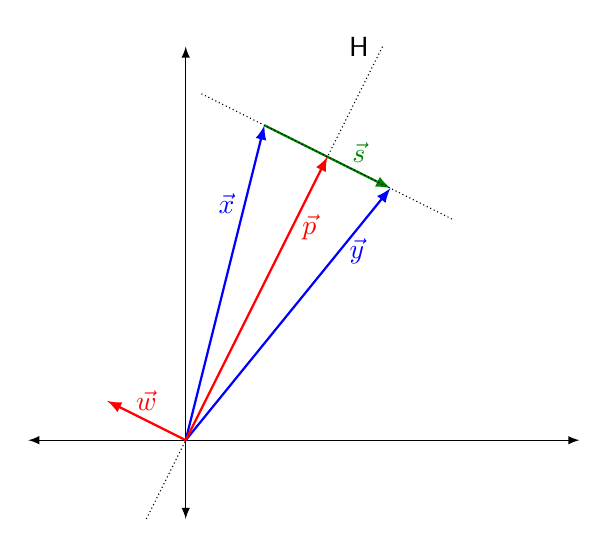
\begin{tikzpicture}[line/.style={>=latex}] 
	\coordinate (w) at (-1, .5);
	\coordinate (wtu) at (1, 2);
	\coordinate (x) at (1, 4);
	\coordinate (wt) at ($2.25/1.25*(wtu)$);
	\coordinate (y) at ($2*(wt)-(x)$);
	\coordinate (V2) at (4, -1);
	\node (HLabel) at (2.2, 5) {$\mathsf{H}$};
	\draw[<->, line] (-2, 0) -- (5, 0);
	\draw[<->, line] (0, -1) -- (0, 5);
	\draw[-, line, densely dotted] (-.5, -1) -- (2.5, 5);
	\draw (HLabel);
	\draw[->, line, color=red, thick] (0, 0) -- node [above] {$\vec{w}$} (w);
	\draw[->, line, color=blue, thick] (0, 0) -- node [left, near end] {$\vec{x}$} (x);
	\draw[->, line, color=blue, thick] (0, 0) -- node [right, near end] {$\vec{y}$} (y);
	\draw[->, line, color=red, thick] (0, 0) -- node [right, near end] {$\vec{p}$} (wt);
	\draw[->, line, color=green!50!black, thick] (x) -- node [above, near end] {$\vec{s}$} (y);
	\draw[-, line, densely dotted] ($2*(x)-(wt)$) -- ($2*(y)-(wt)$);
\end{tikzpicture}
\par
Na figura acima, $p$ como a projeção de $x$ em $\mathsf{H}$ e $s$ é combinação linear de $w$. \\

Projeção de $x$ em $p - x$:\\
\[
	p - x = -\frac{\langle w, x \rangle}{\langle w, w \rangle} w 
\]
\par
temos também:
\[
	s = 2 (p - x) = - 2 \frac{\langle w, x \rangle}{\langle w, w \rangle} w
\]
\par
A reflexão $y$ é $y = x + s$, então:
\[
	y = x - 2 \frac{\langle w, x \rangle}{\langle w, w \rangle} w 
	  = x - 2 \frac{\langle w, x \rangle w }{\langle w, w \rangle}
	  = x - 2 \frac{w \langle w, x \rangle }{\langle w, w \rangle}
\]
\[
	y = x - \frac{2}{w^t w} w.w^t x \Leftrightarrow  
	y = \left(I - \frac{2}{w^t w} w.w^t\right) x
\]
\par
Definimos a transformação linear $H_w$ como:
\[
	H_w(x) = \left(I - \frac{2}{w^t w} w.w^t\right) x
\]

%******************************************************************************
% Decomposição de Schur
%******************************************************************************
\section{Decomposição de Schur}
\begin{theorem}\bref{[Noble,AlgLinApl-pt,1986]}
	Qualquer matriz quadrada $A$, $n \times n$ pode ser reduzida, por uma transformação unitária $P^HAP$, a uma matriz $T$ triangular superior com os autovalores de $A$ sobre a diagonal de $T$. Chamamos $T$ uma forma canônica de Schur para $A$ e a decomposição $A = PTP^H$ é chamada de uma decomposição de Schur de $A$. Se $A$ e seus autovalores são reais, então podemos também tomar $P$ real.
\end{theorem}

Algoritmo:\\
Dado uma matriz quadrada $A$, $n \times n$:
\begin{enumerate}
	\item Achar os $n$ autovalores, $\lambda_1 \dots, \lambda_n$
	\item $A_0 \leftarrow A$.
	\item Para $i = 1, \dots, n - 1$ faça os passos abaixo:
	\begin{enumerate}[label*=\arabic*.]
		\item $Q_i = [ \, v_i \, W_i \, ]$ e $W_i = [ \, w_{i+1} \, \dots \, w_{n} \, ]$ onde $v_i$ é o autovetor \textbf{normalizado} associado a $\lambda_i$ na matriz $A_i$ e $w_{i+1} \, \dots \, w_{n}$ são vetores normais a $v_i$ escolhidos arbitrariamente. (preencha com vetores normais) tal que $Q_i$ seja unitário. Lembrando que $W_i^Hv_i = 0$.
		\item Seja $A_i$ de dimensão $n - i + 1 \times n - i + 1$ e $A_{i+1}$ de dimensão $n - i \times n - i$, faça:
		$A_i$ é matriz de bloco tal que $A_i = \left[\begin{array}{cc}
			\lambda_i &     b_i \\
			        0 & A_{i+1}
		\end{array}\right]$ e  $A_i \leftarrow Q_i^H A_{i-1} Q_i$
	\end{enumerate}
	\item $A_n \leftarrow \lambda_n$ e $P \leftarrow Q_1 Q_2 Q_3 \dots Q_n$
\end{enumerate}

\begin{theorem}\bref{[Noble,AlgLinApl-pt,1986]}
	Uma matriz $A$, $n \times n$ é normal (simétrica real, hermitiana, anti-simétrica, unitária) se e somente se $A$ pode ser reduzida, por uma transformação unitária, a uma forma canônica de Schur diagonal $D = P^HAP$ onde $P$ é unitária e $D$ é diagonal; os autovalores de $A$ estarão sobre a diagonal de $D$. Se $A$ e seus autovalores são reais, então podemos tomar $P$ real e, portanto ortogonal.
\end{theorem}

\begin{theorem}\label{Schur Diagonal}\bref{[Noble,AlgLinApl-pt,1986]}
	Uma matriz $A$, $n \times n$ é normal (simétrica real, hermitiana, anti-simétrica, unitária) se e somente se $A$ pode ser reduzida, por uma transformação unitária, a uma forma canônica de Schur diagonal $D = P^HAP$ onde $P$ é unitária e $D$ é diagonal; os autovalores de $A$ estarão sobre a diagonal de $D$. Se $A$ e seus autovalores são reais, então podemos tomar $P$ real e, portanto ortogonal.
\end{theorem}

\begin{theorem}\bref{[Noble,AlgLinApl-pt,1986]}
	Uma matriz $A$, $n \times n$ é normal (simétrica real, hermitiana, anti-simétrica, unitária) se e somente se $A$ tem um conjunto linearmente independente de $n$ autovetores que podem ser escolhidos de maneira a formar um conjunto ortonormal. Além disso, no caso de uma matriz normal, um autovalor de multiplicidade $s$ tem associado um conjunto ortonormal de $s$ autovetores.
\end{theorem}

%******************************************************************************
% Decomposição em Valores Singulares
%******************************************************************************
\section{Decomposição em Valores Singulares}

\begin{definition}\label{Valores Singulares}\bref{[Noble,AlgLinApl-pt,1986]} Seja a matriz $A$, $m \times n$. As raízes quadradas estritamente positivas de $\sigma_i$ dos autovalores de $A^HA = A^HA$ são chamados de valores singulares de $A$.
\end{definition}

\begin{theorem}\bref{[Noble,AlgLinApl-pt,1986]}
	Suponha a matriz $A$, $m \times n$ tem posto $k$. Existem então números $\sigma_1 \geq \sigma_2 \geq \sigma_3 \geq \dots \sigma_k > 0$, os valores singulares (definição \ref{Valores Singulares}) de $A$ uma matriz unitária $U$, $m \times m$, $U = [ \, u_1 \, u_2 \, u_3 \, \dots u_m \, ]$ e uma matriz unitária $V$, $n \times n$, $V = [ \, v_1 \, v_2 \, v_3 \, \dots v_n \, ]$ tais que:
	\begin{flalign*}
		&\Sigma = U^HAV, \text{ onde: } \left\{\begin{array}{l}
			A \text{ é } m \times n\\
			U \text{ e } V \text{ são } m \times m \text{ e } n \times n \text{ matrizes unitárias }\\
			\Sigma = \left[\begin{array}{cccc}
				\sigma_1 &        0 &  \dots &        0 \\
				       0 & \sigma_2 &  \dots &        0 \\
				  \vdots & \vdots   & \ddots &   \vdots \\
				       0 &        0 &  \dots & \sigma_m \\
				  \vdots & \vdots   & \vdots &   \vdots \\
				       0 &        0 &  \dots &        0
			\end{array}\right] \text{ é } m \times n
		\end{array}\right.&&
	\end{flalign*}
\end{theorem}

Algoritmo:\\
Dado uma matriz quadrada $A$, $m \times n$ e $A = U\Sigma V^H$:
\begin{enumerate}
	\item $A^H A = V\Sigma^HU^HU\Sigma V^H = V(\Sigma^H\Sigma)V^H$, $\sigma^2_i$ é autovalor de $\Sigma^H\Sigma$ (Teorema \ref{Schur Diagonal})
	\item $AA^H = U\Sigma V^HV\Sigma^H U^H = U(\Sigma\Sigma^H)U^H$, $\sigma^2_i$ é autovalor de $\Sigma\Sigma^H$ (Teorema \ref{Schur Diagonal})
	\item Calcular $V = [ \, v_1 \, v_2 \, v_3 \, \dots v_n \, ]$, onde $v_i$ é o autovetor associado a cada $\sigma^2_i$ normalizado da matriz $A^HA$
	\item Calcular $U = [ \, u_1 \, u_2 \, u_3 \, \dots u_m \, ]$, onde $u_i$ é o autovetor associado a cada $\sigma^2_i$ normalizado da matriz $AA^H$
\end{enumerate}

\end{document}

